% Options for packages loaded elsewhere
\PassOptionsToPackage{unicode}{hyperref}
\PassOptionsToPackage{hyphens}{url}
%
\documentclass[
]{article}
\usepackage{amsmath,amssymb}
\usepackage{lmodern}
\usepackage{iftex}
\ifPDFTeX
  \usepackage[T1]{fontenc}
  \usepackage[utf8]{inputenc}
  \usepackage{textcomp} % provide euro and other symbols
\else % if luatex or xetex
  \usepackage{unicode-math}
  \defaultfontfeatures{Scale=MatchLowercase}
  \defaultfontfeatures[\rmfamily]{Ligatures=TeX,Scale=1}
\fi
% Use upquote if available, for straight quotes in verbatim environments
\IfFileExists{upquote.sty}{\usepackage{upquote}}{}
\IfFileExists{microtype.sty}{% use microtype if available
  \usepackage[]{microtype}
  \UseMicrotypeSet[protrusion]{basicmath} % disable protrusion for tt fonts
}{}
\makeatletter
\@ifundefined{KOMAClassName}{% if non-KOMA class
  \IfFileExists{parskip.sty}{%
    \usepackage{parskip}
  }{% else
    \setlength{\parindent}{0pt}
    \setlength{\parskip}{6pt plus 2pt minus 1pt}}
}{% if KOMA class
  \KOMAoptions{parskip=half}}
\makeatother
\usepackage{xcolor}
\IfFileExists{xurl.sty}{\usepackage{xurl}}{} % add URL line breaks if available
\IfFileExists{bookmark.sty}{\usepackage{bookmark}}{\usepackage{hyperref}}
\hypersetup{
  pdftitle={Covid Data and Restrictions - Regression Models},
  hidelinks,
  pdfcreator={LaTeX via pandoc}}
\urlstyle{same} % disable monospaced font for URLs
\usepackage[margin=1in]{geometry}
\usepackage{color}
\usepackage{fancyvrb}
\newcommand{\VerbBar}{|}
\newcommand{\VERB}{\Verb[commandchars=\\\{\}]}
\DefineVerbatimEnvironment{Highlighting}{Verbatim}{commandchars=\\\{\}}
% Add ',fontsize=\small' for more characters per line
\usepackage{framed}
\definecolor{shadecolor}{RGB}{248,248,248}
\newenvironment{Shaded}{\begin{snugshade}}{\end{snugshade}}
\newcommand{\AlertTok}[1]{\textcolor[rgb]{0.94,0.16,0.16}{#1}}
\newcommand{\AnnotationTok}[1]{\textcolor[rgb]{0.56,0.35,0.01}{\textbf{\textit{#1}}}}
\newcommand{\AttributeTok}[1]{\textcolor[rgb]{0.77,0.63,0.00}{#1}}
\newcommand{\BaseNTok}[1]{\textcolor[rgb]{0.00,0.00,0.81}{#1}}
\newcommand{\BuiltInTok}[1]{#1}
\newcommand{\CharTok}[1]{\textcolor[rgb]{0.31,0.60,0.02}{#1}}
\newcommand{\CommentTok}[1]{\textcolor[rgb]{0.56,0.35,0.01}{\textit{#1}}}
\newcommand{\CommentVarTok}[1]{\textcolor[rgb]{0.56,0.35,0.01}{\textbf{\textit{#1}}}}
\newcommand{\ConstantTok}[1]{\textcolor[rgb]{0.00,0.00,0.00}{#1}}
\newcommand{\ControlFlowTok}[1]{\textcolor[rgb]{0.13,0.29,0.53}{\textbf{#1}}}
\newcommand{\DataTypeTok}[1]{\textcolor[rgb]{0.13,0.29,0.53}{#1}}
\newcommand{\DecValTok}[1]{\textcolor[rgb]{0.00,0.00,0.81}{#1}}
\newcommand{\DocumentationTok}[1]{\textcolor[rgb]{0.56,0.35,0.01}{\textbf{\textit{#1}}}}
\newcommand{\ErrorTok}[1]{\textcolor[rgb]{0.64,0.00,0.00}{\textbf{#1}}}
\newcommand{\ExtensionTok}[1]{#1}
\newcommand{\FloatTok}[1]{\textcolor[rgb]{0.00,0.00,0.81}{#1}}
\newcommand{\FunctionTok}[1]{\textcolor[rgb]{0.00,0.00,0.00}{#1}}
\newcommand{\ImportTok}[1]{#1}
\newcommand{\InformationTok}[1]{\textcolor[rgb]{0.56,0.35,0.01}{\textbf{\textit{#1}}}}
\newcommand{\KeywordTok}[1]{\textcolor[rgb]{0.13,0.29,0.53}{\textbf{#1}}}
\newcommand{\NormalTok}[1]{#1}
\newcommand{\OperatorTok}[1]{\textcolor[rgb]{0.81,0.36,0.00}{\textbf{#1}}}
\newcommand{\OtherTok}[1]{\textcolor[rgb]{0.56,0.35,0.01}{#1}}
\newcommand{\PreprocessorTok}[1]{\textcolor[rgb]{0.56,0.35,0.01}{\textit{#1}}}
\newcommand{\RegionMarkerTok}[1]{#1}
\newcommand{\SpecialCharTok}[1]{\textcolor[rgb]{0.00,0.00,0.00}{#1}}
\newcommand{\SpecialStringTok}[1]{\textcolor[rgb]{0.31,0.60,0.02}{#1}}
\newcommand{\StringTok}[1]{\textcolor[rgb]{0.31,0.60,0.02}{#1}}
\newcommand{\VariableTok}[1]{\textcolor[rgb]{0.00,0.00,0.00}{#1}}
\newcommand{\VerbatimStringTok}[1]{\textcolor[rgb]{0.31,0.60,0.02}{#1}}
\newcommand{\WarningTok}[1]{\textcolor[rgb]{0.56,0.35,0.01}{\textbf{\textit{#1}}}}
\usepackage{graphicx}
\makeatletter
\def\maxwidth{\ifdim\Gin@nat@width>\linewidth\linewidth\else\Gin@nat@width\fi}
\def\maxheight{\ifdim\Gin@nat@height>\textheight\textheight\else\Gin@nat@height\fi}
\makeatother
% Scale images if necessary, so that they will not overflow the page
% margins by default, and it is still possible to overwrite the defaults
% using explicit options in \includegraphics[width, height, ...]{}
\setkeys{Gin}{width=\maxwidth,height=\maxheight,keepaspectratio}
% Set default figure placement to htbp
\makeatletter
\def\fps@figure{htbp}
\makeatother
\setlength{\emergencystretch}{3em} % prevent overfull lines
\providecommand{\tightlist}{%
  \setlength{\itemsep}{0pt}\setlength{\parskip}{0pt}}
\setcounter{secnumdepth}{-\maxdimen} % remove section numbering
\usepackage{booktabs}
\usepackage{longtable}
\usepackage{array}
\usepackage{multirow}
\usepackage{wrapfig}
\usepackage{float}
\usepackage{colortbl}
\usepackage{pdflscape}
\usepackage{tabu}
\usepackage{threeparttable}
\usepackage{threeparttablex}
\usepackage[normalem]{ulem}
\usepackage{makecell}
\usepackage{xcolor}
\ifLuaTeX
  \usepackage{selnolig}  % disable illegal ligatures
\fi

\title{Covid Data and Restrictions - Regression Models}
\author{}
\date{\vspace{-2.5em}}

\begin{document}
\maketitle

\hypertarget{european-countries---2020-12-30}{%
\section{\texorpdfstring{\textbf{European Countries -
2020-12-30}}{European Countries - 2020-12-30}}\label{european-countries---2020-12-30}}

\hypertarget{maps}{%
\subsubsection{Maps}\label{maps}}

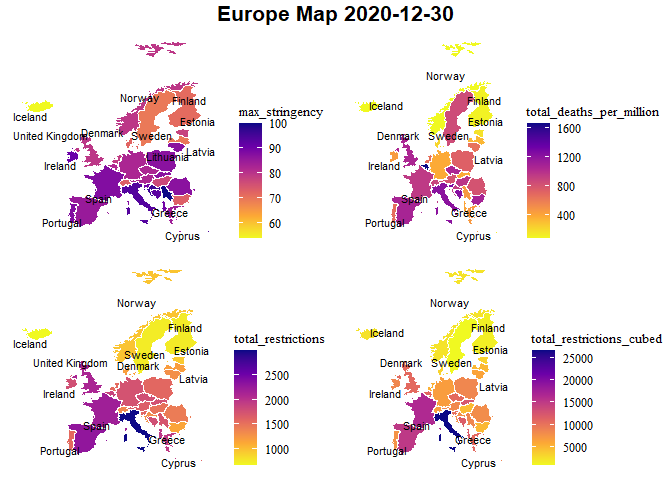
\includegraphics{03_Analysis_files/figure-latex/unnamed-chunk-4-1.pdf}

\hypertarget{correlations---total-covid-deaths-per-million}{%
\subsubsection{Correlations - total covid deaths per
million}\label{correlations---total-covid-deaths-per-million}}

\begin{table}

\caption{\label{tab:unnamed-chunk-5}Correlation - Europe - Total deaths per million - 2020-12-30}
\centering
\begin{tabular}[t]{l|r}
\hline
Variable & total\_deaths\_per\_million\\
\hline
longitude & -0.4023597\\
\hline
latitude & -0.3742363\\
\hline
date\_first\_death\_days & -0.3611278\\
\hline
human\_development\_index & -0.1608582\\
\hline
gdp\_per\_capita & -0.1310446\\
\hline
diabetes\_prevalence & -0.0401322\\
\hline
cardiovasc\_death\_rate & -0.0199638\\
\hline
male\_smokers & 0.0051781\\
\hline
life\_expectancy & 0.0151471\\
\hline
extreme\_poverty & 0.1256898\\
\hline
max\_stringency & 0.2588952\\
\hline
female\_smokers & 0.2816485\\
\hline
aged\_65\_older & 0.2944033\\
\hline
population\_density & 0.3844200\\
\hline
median\_age & 0.4028280\\
\hline
total\_restrictions & 0.4960606\\
\hline
total\_restrictions\_cubed & 0.5063557\\
\hline
total\_cases\_per\_million & 0.6298464\\
\hline
people\_fully\_vaccinated\_per\_hundred & NA\\
\hline
\end{tabular}
\end{table}

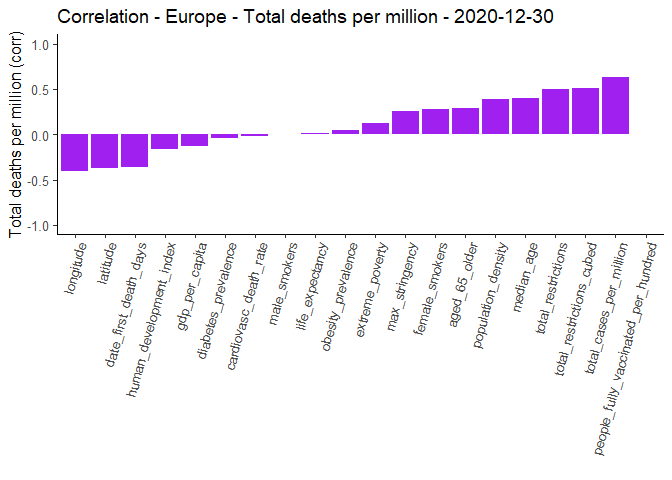
\includegraphics{03_Analysis_files/figure-latex/unnamed-chunk-5-1.pdf}
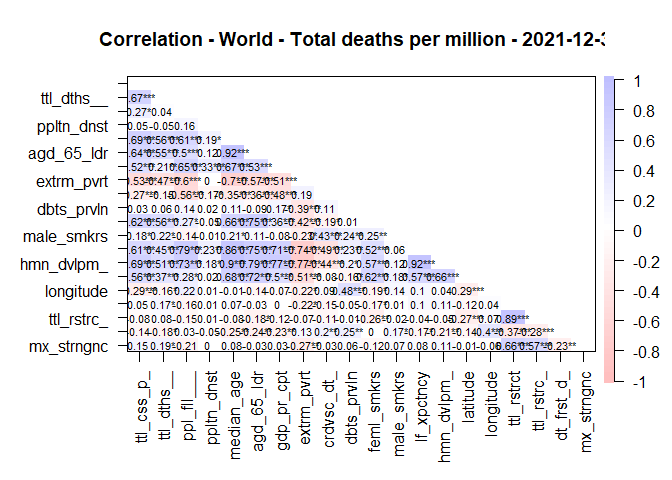
\includegraphics{03_Analysis_files/figure-latex/unnamed-chunk-5-2.pdf}

\hypertarget{scatter-plots---total-covid-deaths-per-million-vs.-stringency-total_restrictions-cubed}{%
\subsubsection{Scatter plots - total covid deaths per million
vs.~stringency / total\_restrictions
cubed}\label{scatter-plots---total-covid-deaths-per-million-vs.-stringency-total_restrictions-cubed}}

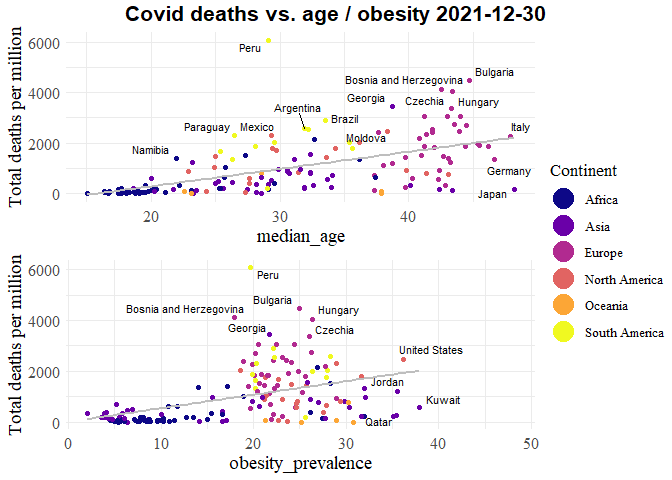
\includegraphics{03_Analysis_files/figure-latex/unnamed-chunk-6-1.pdf}
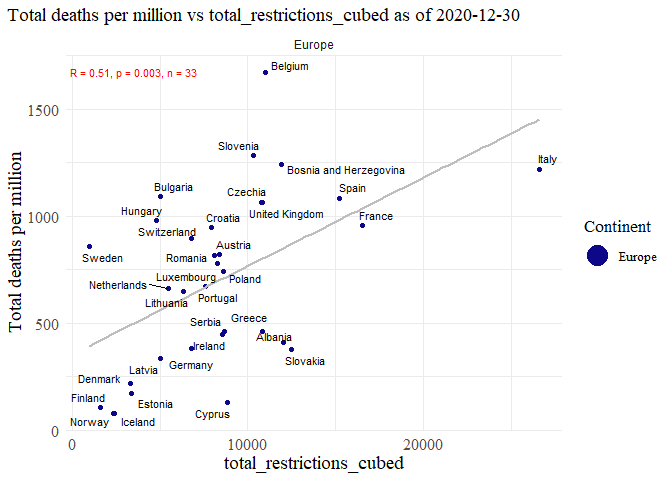
\includegraphics{03_Analysis_files/figure-latex/unnamed-chunk-6-2.pdf}

\hypertarget{regression}{%
\subsubsection{Regression}\label{regression}}

\hypertarget{replication-of-regression-analysis-from-lally-2022-paper.}{%
\subparagraph{\texorpdfstring{Replication of regression analysis from
\href{https://link.springer.com/content/pdf/10.1007/s40592-021-00148-y.pdf}{Lally
(2022)}
paper.}{Replication of regression analysis from Lally (2022) paper.}}\label{replication-of-regression-analysis-from-lally-2022-paper.}}

\begin{table}
\centering
\begin{tabular}[t]{l}
\hline
regression\\
\hline
\\
\hline
Call:\\
\hline
lm(formula = total\_deaths\_per\_million \textasciitilde{} max\_stringency + population\_density +\\
\hline
date\_first\_death\_days, data = df)\\
\hline
\\
\hline
Residuals:\\
\hline
Min      1Q  Median      3Q     Max\\
\hline
-571.81 -298.20   -5.26  219.37  684.67\\
\hline
\\
\hline
Coefficients:\\
\hline
Estimate Std. Error t value Pr(>|t|)\\
\hline
(Intercept)            68.6981   623.5790   0.110    0.913\\
\hline
max\_stringency          9.6139     6.9077   1.392    0.175\\
\hline
population\_density      1.0600     0.6546   1.619    0.116\\
\hline
date\_first\_death\_days -10.3515     7.0974  -1.458    0.155\\
\hline
\\
\hline
Residual standard error: 368.2 on 29 degrees of freedom\\
\hline
Multiple R-squared:  0.2552,    Adjusted R-squared:  0.1782\\
\hline
F-statistic: 3.313 on 3 and 29 DF,  p-value: 0.03376\\
\hline
\\
\hline
\end{tabular}
\end{table}

\begin{table}
\centering
\begin{tabular}[t]{l}
\hline
regression\\
\hline
\\
\hline
Call:\\
\hline
lm(formula = total\_deaths\_per\_million \textasciitilde{} total\_restrictions +\\
\hline
population\_density + date\_first\_death\_days, data = df)\\
\hline
\\
\hline
Residuals:\\
\hline
Min      1Q  Median      3Q     Max\\
\hline
-527.35 -293.07  -19.61  223.81  683.79\\
\hline
\\
\hline
Coefficients:\\
\hline
Estimate Std. Error t value Pr(>|t|)\\
\hline
(Intercept)           288.4651   386.7476   0.746   0.4617\\
\hline
total\_restrictions      0.2998     0.1564   1.916   0.0652 .\\
\hline
population\_density      0.7191     0.6688   1.075   0.2911\\
\hline
date\_first\_death\_days  -5.1813     7.4667  -0.694   0.4933\\
\hline
---\\
\hline
Signif. codes:  0 '***' 0.001 '**' 0.01 '*' 0.05 '.' 0.1 ' ' 1\\
\hline
\\
\hline
Residual standard error: 358.3 on 29 degrees of freedom\\
\hline
Multiple R-squared:  0.2948,    Adjusted R-squared:  0.2218\\
\hline
F-statistic: 4.041 on 3 and 29 DF,  p-value: 0.01622\\
\hline
\\
\hline
\end{tabular}
\end{table}

\hypertarget{european-countries---2021-12-30}{%
\section{\texorpdfstring{\textbf{European Countries -
2021-12-30}}{European Countries - 2021-12-30}}\label{european-countries---2021-12-30}}

\hypertarget{maps-1}{%
\subsubsection{Maps}\label{maps-1}}

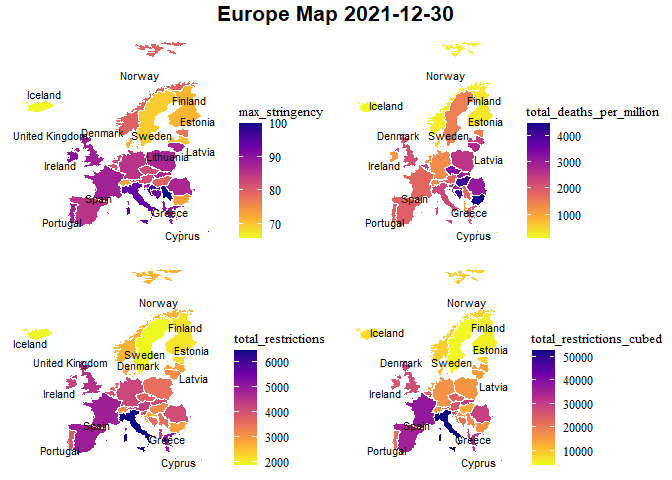
\includegraphics{03_Analysis_files/figure-latex/unnamed-chunk-8-1.pdf}

\hypertarget{correlations}{%
\subsubsection{Correlations}\label{correlations}}

\begin{table}

\caption{\label{tab:unnamed-chunk-9}Correlation - Europe - Total deaths per million - 2021-12-30}
\centering
\begin{tabular}[t]{l|r}
\hline
Variable & total\_deaths\_per\_million\\
\hline
people\_fully\_vaccinated\_per\_hundred & -0.7221438\\
\hline
life\_expectancy & -0.6334930\\
\hline
human\_development\_index & -0.6250602\\
\hline
gdp\_per\_capita & -0.5305191\\
\hline
latitude & -0.3964205\\
\hline
population\_density & -0.0207148\\
\hline
diabetes\_prevalence & 0.1656193\\
\hline
total\_restrictions & 0.1698663\\
\hline
longitude & 0.1792136\\
\hline
date\_first\_death\_days & 0.1833453\\
\hline
aged\_65\_older & 0.2150767\\
\hline
total\_restrictions\_cubed & 0.2404483\\
\hline
max\_stringency & 0.2584739\\
\hline
total\_cases\_per\_million & 0.2759254\\
\hline
extreme\_poverty & 0.2842681\\
\hline
median\_age & 0.4245012\\
\hline
male\_smokers & 0.4494477\\
\hline
female\_smokers & 0.4887887\\
\hline
cardiovasc\_death\_rate & 0.6004901\\
\hline
\end{tabular}
\end{table}

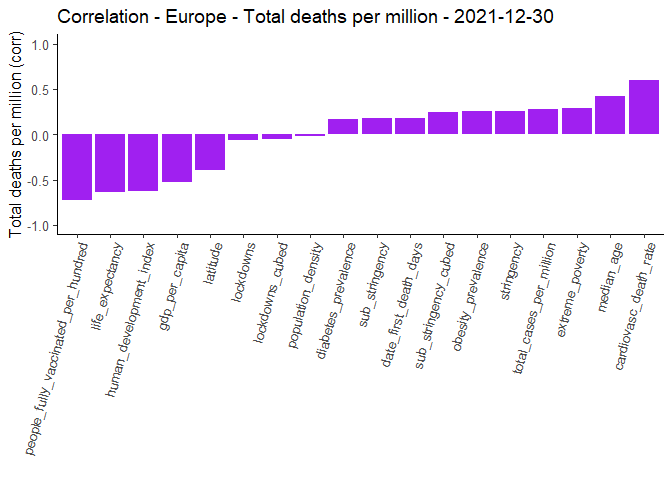
\includegraphics{03_Analysis_files/figure-latex/unnamed-chunk-9-1.pdf}
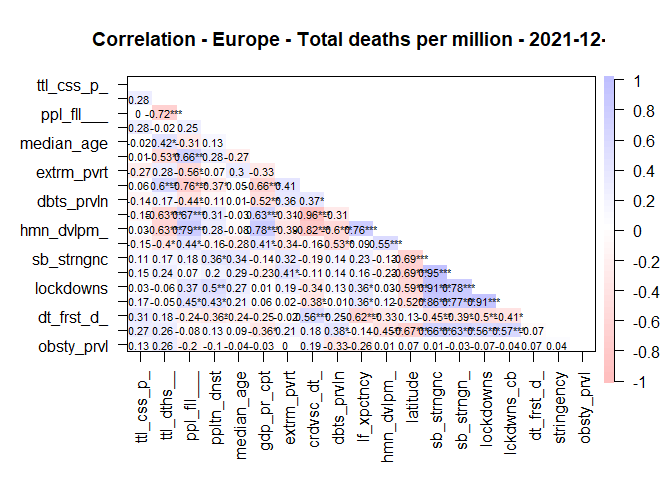
\includegraphics{03_Analysis_files/figure-latex/unnamed-chunk-9-2.pdf}
\#\#\# Scatter plots - total deaths per million vs.~stringency / total
restrictions cubed

\begin{Shaded}
\begin{Highlighting}[]
\FunctionTok{country\_scatter}\NormalTok{(df\_europe\_20211230,}\StringTok{"max\_stringency"}\NormalTok{,}\StringTok{\textquotesingle{}yes\textquotesingle{}}\NormalTok{)}
\end{Highlighting}
\end{Shaded}

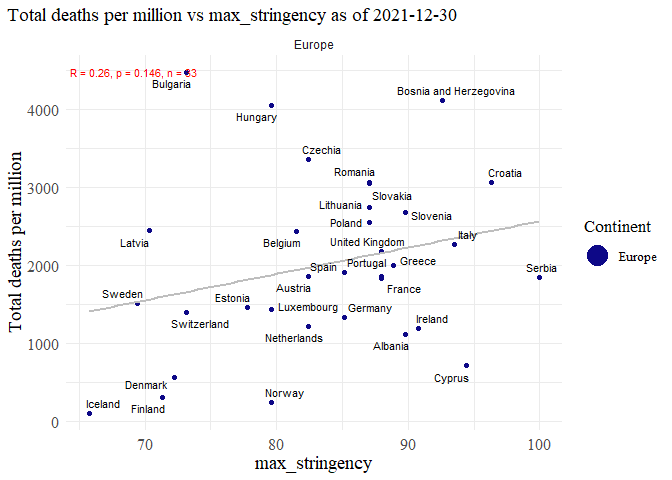
\includegraphics{03_Analysis_files/figure-latex/unnamed-chunk-10-1.pdf}

\begin{Shaded}
\begin{Highlighting}[]
\FunctionTok{country\_scatter}\NormalTok{(df\_europe\_20211230,}\StringTok{"total\_restrictions\_cubed"}\NormalTok{,}\StringTok{\textquotesingle{}yes\textquotesingle{}}\NormalTok{)}
\end{Highlighting}
\end{Shaded}

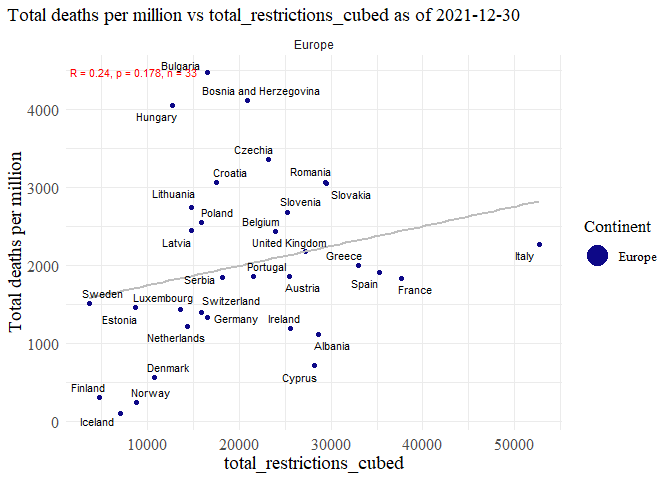
\includegraphics{03_Analysis_files/figure-latex/unnamed-chunk-10-2.pdf}

\hypertarget{regression-1}{%
\subsubsection{Regression}\label{regression-1}}

\begin{table}
\centering
\begin{tabular}[t]{l}
\hline
regression\\
\hline
\\
\hline
Call:\\
\hline
lm(formula = total\_deaths\_per\_million \textasciitilde{} max\_stringency + population\_density +\\
\hline
date\_first\_death\_days, data = df)\\
\hline
\\
\hline
Residuals:\\
\hline
Min      1Q  Median      3Q     Max\\
\hline
-1944.0  -643.8   106.9   463.3  2917.0\\
\hline
\\
\hline
Coefficients:\\
\hline
Estimate Std. Error t value Pr(>|t|)\\
\hline
(Intercept)           -1631.0135  2063.0365  -0.791    0.436\\
\hline
max\_stringency           35.3352    23.1630   1.526    0.138\\
\hline
population\_density        0.1942     1.9565   0.099    0.922\\
\hline
date\_first\_death\_days    23.3921    21.1191   1.108    0.277\\
\hline
\\
\hline
Residual standard error: 1096 on 29 degrees of freedom\\
\hline
Multiple R-squared:  0.1075,    Adjusted R-squared:  0.01517\\
\hline
F-statistic: 1.164 on 3 and 29 DF,  p-value: 0.3403\\
\hline
\\
\hline
\end{tabular}
\end{table}

\begin{table}
\centering
\begin{tabular}[t]{l}
\hline
regression\\
\hline
\\
\hline
Call:\\
\hline
lm(formula = total\_deaths\_per\_million \textasciitilde{} total\_restrictions +\\
\hline
population\_density + date\_first\_death\_days, data = df)\\
\hline
\\
\hline
Residuals:\\
\hline
Min      1Q  Median      3Q     Max\\
\hline
-1941.7  -471.0  -140.2   517.0  2816.1\\
\hline
\\
\hline
Coefficients:\\
\hline
Estimate Std. Error t value Pr(>|t|)\\
\hline
(Intercept)           -271.9398  1233.4326  -0.220    0.827\\
\hline
total\_restrictions       0.3574     0.2232   1.601    0.120\\
\hline
population\_density      -0.2535     1.9975  -0.127    0.900\\
\hline
date\_first\_death\_days   36.0393    22.6349   1.592    0.122\\
\hline
\\
\hline
Residual standard error: 1092 on 29 degrees of freedom\\
\hline
Multiple R-squared:  0.1141,    Adjusted R-squared:  0.0225\\
\hline
F-statistic: 1.246 on 3 and 29 DF,  p-value: 0.3113\\
\hline
\\
\hline
\end{tabular}
\end{table}

\hypertarget{european-countries---2022-05-20}{%
\section{\texorpdfstring{\textbf{European Countries -
2022-05-20}}{European Countries - 2022-05-20}}\label{european-countries---2022-05-20}}

\hypertarget{maps-2}{%
\subsubsection{Maps}\label{maps-2}}

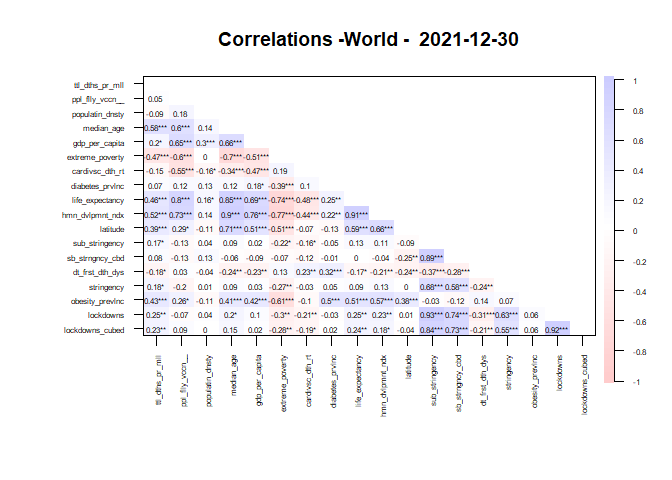
\includegraphics{03_Analysis_files/figure-latex/unnamed-chunk-12-1.pdf}

\hypertarget{correlations-1}{%
\subsubsection{Correlations}\label{correlations-1}}

\begin{table}

\caption{\label{tab:unnamed-chunk-13}Correlation - Europe - Total deaths per million - 2022-05-20}
\centering
\begin{tabular}[t]{l|r}
\hline
Variable & total\_deaths\_per\_million\\
\hline
people\_fully\_vaccinated\_per\_hundred & -0.7388776\\
\hline
life\_expectancy & -0.6576227\\
\hline
human\_development\_index & -0.6355075\\
\hline
gdp\_per\_capita & -0.5597761\\
\hline
latitude & -0.3810561\\
\hline
total\_cases\_per\_million & -0.3568545\\
\hline
population\_density & -0.0911554\\
\hline
diabetes\_prevalence & 0.1440602\\
\hline
total\_restrictions & 0.1518520\\
\hline
date\_first\_death\_days & 0.2167162\\
\hline
total\_restrictions\_cubed & 0.2278267\\
\hline
aged\_65\_older & 0.2401198\\
\hline
longitude & 0.2445521\\
\hline
max\_stringency & 0.2483456\\
\hline
extreme\_poverty & 0.2540468\\
\hline
median\_age & 0.4328025\\
\hline
male\_smokers & 0.4732112\\
\hline
female\_smokers & 0.5176944\\
\hline
cardiovasc\_death\_rate & 0.6221463\\
\hline
\end{tabular}
\end{table}

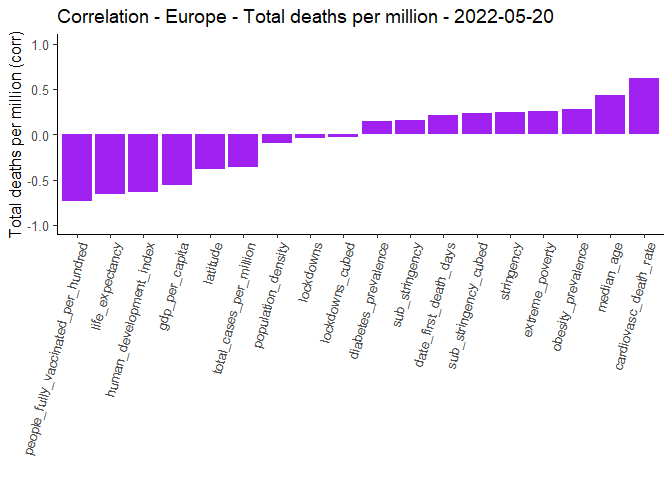
\includegraphics{03_Analysis_files/figure-latex/unnamed-chunk-13-1.pdf}
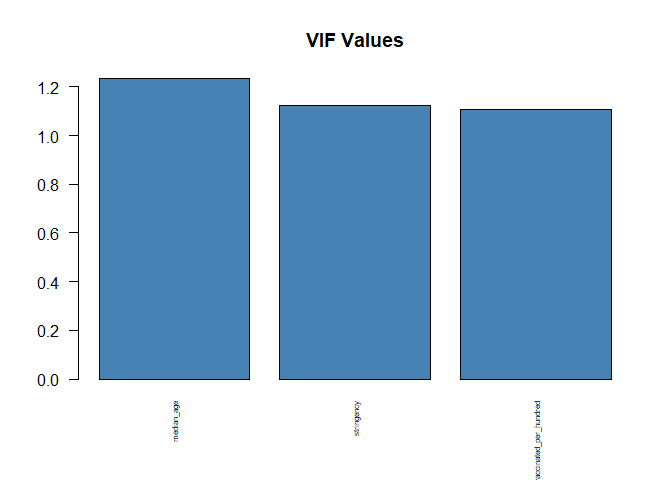
\includegraphics{03_Analysis_files/figure-latex/unnamed-chunk-13-2.pdf}

\hypertarget{scatter-plots---total-deaths-per-million-vs.-stringency-total-restrictions-cubed}{%
\subsubsection{Scatter plots - total deaths per million vs.~stringency /
total restrictions
cubed}\label{scatter-plots---total-deaths-per-million-vs.-stringency-total-restrictions-cubed}}

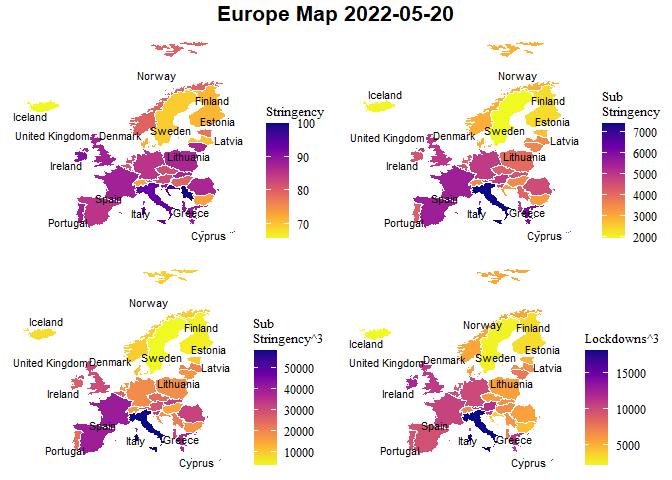
\includegraphics{03_Analysis_files/figure-latex/unnamed-chunk-14-1.pdf}
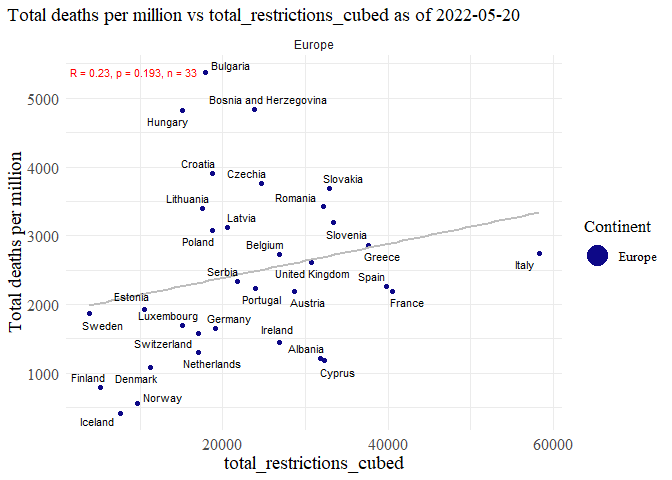
\includegraphics{03_Analysis_files/figure-latex/unnamed-chunk-14-2.pdf}

\hypertarget{regression-2}{%
\subsubsection{Regression}\label{regression-2}}

\begin{table}
\centering
\begin{tabular}[t]{l}
\hline
regression\\
\hline
\\
\hline
Call:\\
\hline
lm(formula = total\_deaths\_per\_million \textasciitilde{} max\_stringency + population\_density +\\
\hline
date\_first\_death\_days, data = df)\\
\hline
\\
\hline
Residuals:\\
\hline
Min      1Q  Median      3Q     Max\\
\hline
-2022.0  -685.1    10.5   558.9  3369.1\\
\hline
\\
\hline
Coefficients:\\
\hline
Estimate Std. Error t value Pr(>|t|)\\
\hline
(Intercept)           -1552.3293  2306.2900  -0.673    0.506\\
\hline
max\_stringency           39.6024    25.8942   1.529    0.137\\
\hline
population\_density       -0.5615     2.1872  -0.257    0.799\\
\hline
date\_first\_death\_days    27.5147    23.6093   1.165    0.253\\
\hline
\\
\hline
Residual standard error: 1225 on 29 degrees of freedom\\
\hline
Multiple R-squared:  0.1183,    Adjusted R-squared:  0.0271\\
\hline
F-statistic: 1.297 on 3 and 29 DF,  p-value: 0.2942\\
\hline
\\
\hline
\end{tabular}
\end{table}

\begin{table}
\centering
\begin{tabular}[t]{l}
\hline
regression\\
\hline
\\
\hline
Call:\\
\hline
lm(formula = total\_deaths\_per\_million \textasciitilde{} total\_restrictions +\\
\hline
population\_density + date\_first\_death\_days, data = df)\\
\hline
\\
\hline
Residuals:\\
\hline
Min      1Q  Median      3Q     Max\\
\hline
-2030.3  -613.8  -199.8   502.2  3254.6\\
\hline
\\
\hline
Coefficients:\\
\hline
Estimate Std. Error t value Pr(>|t|)\\
\hline
(Intercept)             88.6112  1324.1476   0.067    0.947\\
\hline
total\_restrictions       0.3345     0.2092   1.599    0.121\\
\hline
population\_density      -1.0599     2.2336  -0.475    0.639\\
\hline
date\_first\_death\_days   39.8655    24.9225   1.600    0.121\\
\hline
\\
\hline
Residual standard error: 1221 on 29 degrees of freedom\\
\hline
Multiple R-squared:  0.1244,    Adjusted R-squared:  0.03381\\
\hline
F-statistic: 1.373 on 3 and 29 DF,  p-value: 0.2706\\
\hline
\\
\hline
\end{tabular}
\end{table}

\begin{table}
\centering
\begin{tabular}[t]{l}
\hline
regression\\
\hline
\\
\hline
Call:\\
\hline
lm(formula = total\_deaths\_per\_million \textasciitilde{} total\_restrictions\_cubed +\\
\hline
people\_fully\_vaccinated\_per\_hundred + life\_expectancy + latitude,\\
\hline
data = df\_europe\_20220520)\\
\hline
\\
\hline
Residuals:\\
\hline
Min      1Q  Median      3Q     Max\\
\hline
-1209.1  -230.4  -125.4   309.3   832.6\\
\hline
\\
\hline
Coefficients:\\
\hline
Estimate  Std. Error t value  Pr(>|t|)\\
\hline
(Intercept)                         26744.46858  4922.02183   5.434 0.0000552\\
\hline
total\_restrictions\_cubed                0.02117     0.01293   1.636   0.12126\\
\hline
people\_fully\_vaccinated\_per\_hundred   -22.61953    12.58687  -1.797   0.09122\\
\hline
life\_expectancy                      -247.08346    62.70359  -3.940   0.00117\\
\hline
latitude                              -65.98226    24.30157  -2.715   0.01529\\
\hline
\\
\hline
(Intercept)                         ***\\
\hline
total\_restrictions\_cubed\\
\hline
people\_fully\_vaccinated\_per\_hundred .\\
\hline
life\_expectancy                     **\\
\hline
latitude                            *\\
\hline
---\\
\hline
Signif. codes:  0 '***' 0.001 '**' 0.01 '*' 0.05 '.' 0.1 ' ' 1\\
\hline
\\
\hline
Residual standard error: 495.7 on 16 degrees of freedom\\
\hline
(12 observations deleted due to missingness)\\
\hline
Multiple R-squared:  0.8334,    Adjusted R-squared:  0.7918\\
\hline
F-statistic: 20.01 on 4 and 16 DF,  p-value: 0.000004549\\
\hline
\\
\hline
\end{tabular}
\end{table}

\hypertarget{countries-in-the-analysis}{%
\paragraph{Countries in the analysis}\label{countries-in-the-analysis}}

\begin{table}

\caption{\label{tab:unnamed-chunk-16}Countries in analysis (n = 33)}
\centering
\begin{tabular}[t]{l}
\hline
Countries\\
\hline
Austria\\
\hline
Albania\\
\hline
Belgium\\
\hline
Bosnia and Herzegovina\\
\hline
Bulgaria\\
\hline
Croatia\\
\hline
Cyprus\\
\hline
Czechia\\
\hline
Denmark\\
\hline
Estonia\\
\hline
Finland\\
\hline
France\\
\hline
Germany\\
\hline
Greece\\
\hline
Hungary\\
\hline
Iceland\\
\hline
Ireland\\
\hline
Italy\\
\hline
Latvia\\
\hline
Lithuania\\
\hline
Luxembourg\\
\hline
Netherlands\\
\hline
Norway\\
\hline
Poland\\
\hline
Portugal\\
\hline
Romania\\
\hline
Serbia\\
\hline
Slovakia\\
\hline
Slovenia\\
\hline
Spain\\
\hline
Sweden\\
\hline
Switzerland\\
\hline
United Kingdom\\
\hline
\end{tabular}
\end{table}

\hypertarget{data-sources}{%
\subsubsection{Data sources:}\label{data-sources}}

\begin{itemize}
\tightlist
\item
  \href{https://covid.ourworldindata.org/data/owid-covid-data.csv}{Our
  World in Data}
\item
  \href{https://raw.githubusercontent.com/OxCGRT/covid-policy-tracker/master/data/OxCGRT_latest.csv}{The
  Oxford COVID-19 Government Response Tracker}
\item
  \href{https://raw.githubusercontent.com/albertyw/avenews/master/old/data/average-latitude-longitude-countries.csv}{Average
  latitude \& longitude for Countries}
\end{itemize}

\end{document}
